\documentclass [10pt,letterpaper]{report}
%\documentclass[10pt,letterpaper]{article}
%\documentclass[10pt,letterpaper,twocolumn]{article}
%
%\documentclass[10pt,letterpaper,twocolumn]{report}
%\documentclass[10pt,letterpaper]{report}
%
%\usepackage[greek,english]{babel}
\usepackage[greek,english]{babel}
\usepackage[T1]{fontenc}
\usepackage{graphicx}
\usepackage{color}
\usepackage{wrapfig}


\textheight     =  8.4in
\textwidth      =  6.8in
%\parindent      =  0.0cm

\topmargin      =  -0.2in
\oddsidemargin  =  -0.2in
\evensidemargin =  -0.2in
%\hoffset        =  0.0cm
%\voffset        =  0.0cm

\newcommand{\nuSolve}{\greektext n\latintext Solve}
\newcommand{\thisVersion}{0.7.2}

\graphicspath{{graphics/}}

\begin{document}

\title{vgosDbProcLogs-\thisVersion{}: User Guide}

\author{
Sergei Bolotin,
Karen Baver,
John Gipson,
David Gordon,
Daniel MacMillan
}

\date{\today}


\maketitle

\tableofcontents



\def\leftSp      {48mm}
\def\riteSp     {113mm}


\chapter{Introduction}
\label{intro}

This document describes how to use the utility vgosDbProcLogs.

The utility extracts from station log files cable calibration data and
meteorological parameters and stores them in vgosDb format.

The utility vgosDbProcLogs is distributed in nusolve package that contains \nuSolve{}
software and utilities vgosDbMake, vgosDbCalc and vgosDbProcLogs. Each of the
utilities has its own version number that can differ from distribution version,
e.g., the first release of vgosDbProcLogs-0.1.0 appeared in nusolve-0.2.11 package.

The guide covers \thisVersion{} version of the software. Since the vgosDbProcLogs
is a simple utility we do not expect large modifications of the User Guide version
from version.


\section{Requirements}
\label{intro_reqs}

See \emph{\nuSolve{} User Guide} for the requirements.


\section{Changes from previous versions}
\label{intro_changes}

This section was added in 0.5.0 version of the nusolve distribution
(version 0.3.0 of the vgosDbProcLogs user guide). It covers changes in
the software and the user guide.


\subsection{Changes in version 0.7.3}
Strict treatment of type of intput files is implemented.

\subsection{Changes in version 0.7.2}
Nothing essential was changed.

\subsection{Changes in version 0.7.1}
Nothing essential was changed.

\subsection{Changes in version 0.7.0}
Support of version 2 of masterfile and new database naming convention is added.

\subsection{Changes in version 0.6.6}
Few bug fixes in handling of cable calibration data.

\subsection{Changes in version 0.6.5}
The utility collects all available cable calibration corrections from various
sources: FS log file, CDMS and PCMT. It accumulates these data in a separate
netCDF files.


\subsection{Changes in version 0.6.4}
The command line arguments parser has switched to ARGP from GNU C Library.

A command line option ("-o") was added to set an order of meteorological
parameters in a log file. An obsolete option "-f" was removed.
See chapter \emph{\ref{chapter_invokation} Invoking vgosDbProcLogs} for details.

Parsing tsys records for legacy stations currently is disabled (log2ant should
be used instead), the command line options that control tsys processing are
ignored.

Few misprints were fixed.


\subsection{Changes in version 0.6.3}
A command line option {\tt -d} is added to alter a directory with input files.
It could be useful to specify path to log or PCMT files that are not in standard
place. Chapter \emph{\ref{chapter_invokation} Invoking vgosDbProcLogs} was modified
to reflect the changes.


\subsection{Changes in version 0.6.2}
Nothing essential was changed.


\subsection{Changes in version 0.6.1}
Nothing essential was changed.


\subsection{Changes in version 0.6.0}
New command line arguments were added, see the chapter
\emph{\ref{chapter_invokation} Invoking vgosDbProcLogs} for details.

A dry mode has been implemented, the software reads input files, creates and fills
all internal structures, but nothing is written.

Dealing with locale has been altered. Unfortunately, people do not read the manuals,
as a result their locale set up conflicts with HOPS parsing of fringe files. Now,
by default the locale is set to "C" after the utility is started. There are options
to configure this feature in the wizard as well as a command line argument.

Version of the utility jumped from 0.4.4. to 0.6.0.

\subsection{Changes in version 0.4.4}
Nothing essential was modified.

\subsection{Changes in version 0.4.3}
This update contains bug fixes.

\subsection{Changes in version 0.4.2}
In this version behavior of vgosDbProcLogs has been modified: if the environment
variable <<\$DISPLAY>> is not set, calls to pop up windows with error messages are
suppressed. Also, during creation of the wrapper file name, the attribute
<<\_i[Institution]>> will be added. To suppress the last option, the short
abbreviation of the affiliation should not be set (e.g., on the Fig.~\ref{fig-wizzard-3}
put an empty string instead of <<GSFC>>).

A warning about permanently increase of the log file size was added to the section
\emph{\ref{config_logger} Setting options of the logger}.

The order of processing input files has been changed from log files,
CDMS, PCMT and meteo data to CDMS, PCMT, meteo data and log files;
see \emph{\ref{sect_command_line_arguments} Command line arguments}.

A Section~\emph{\ref{config_cablecal_signs} Setting default cable calibration signs}
was added to describe set up of the default cable calibration signs.

Configuration of use meteo data in RINEX format is added and is described in the
Section \emph{\ref{config_rinex} Setting RINEX files}.


\subsection{Changes in version 0.4.1}
The command line options {\tt -p} and {\tt -W} are added in this version, see
the chapter \emph{\ref{chapter_invokation} Invoking vgosDbProcLogs}.

A section \emph{\ref{sect_systemwide_settings} Using system-wide settings} is added.

Description how to use RINEX files with meteorological data for some VLBI
stations is added as a section \emph{\ref{sect_using_rinex_files} Using RINEX files}.

The URL of software distribution has been updated in the chapter
\emph{\ref{chapt_concluding_remark} Concluding remark}.



\subsection{Changes in version 0.4.0}
The software is capable to process external files with cable calibration
and meteorological data, also, a user can specify what station(s) it
should process. These changes are covered in the
chapter \emph{\ref{chapter_invokation} Invoking vgosDbProcLogs}.


\subsection{Changes in version 0.3.0}
The utility is able to read an alternative version of master files. The
use of the local master files is described in the section
\emph{\ref{config_paths} Setting paths to data}.

The sections \emph{\ref{intro_reqs} Requirements} and
\emph{\ref{intro_changes} Changes from previous versions} were added to
the chapter \emph{\ref{intro} Introductions}.






%%%%%%%%%%%%%%%%%%%%%%%%%%%%%%%%%%%%%%%%%%%%%%%%%%%%%%%%%%%%%%%%%%%%%%%%%%%%%%
%
%
\chapter{Installation}

The source codes of vgosDbProcLogs is distributed along with \nuSolve{}
software. The latest stable version of the software one can find at
{\tt https://sourceforge.net/projects/nusolve} with a name like
{\tt nusolve-1.2.3.tar.gz}. Since the software is still in an active
development phase, we recommend you use the latest version.

The utility is compiled during compilation of \nuSolve{} software, there
is no any additional option to turn its compilation on or modify
somehow. Please, refer to \nuSolve{} User Guide how to configure,
compile and install the software.


%%%%%%%%%%%%%%%%%%%%%%%%%%%%%%%%%%%%%%%%%%%%%%%%%%%%%%%%%%%%%%%%%%%%%%%%%%%%%%
%
%
\chapter{Invoking vgosDbProcLogs}

%
%
%
% Where to get log files?
%
% http://www.vlba.nrao.edu/astro/VOBS/IVS/
%
%
%
%
%



\label{chapter_invokation}
To invoke vgosDbProcLogs just type (specifying if necessary the full path
to the executable) program name and a wrapper file of a VLBI session:
\begin{verbatim}
> vgosDbProcLogs <wrapper file>
\end{verbatim}
\noindent
Where {\sl <wrapper file>} is a path and name of the session wrapper file.
The wrapper file path can be in absolute (i.e., starting with <</>> char)
or relative form. If the relative form is used, then the software searches
for files starting from a directory which is specified in
{\sl Path to VgosDb files} field of the setup wizard (see Section~\ref{config_paths}).

For example, to extract information from station log files of a VLBI session
{\sl eur136} and store it in vgosDb format I can execute vgosDbProcLogs in
the following way:
\begin{verbatim}
> vgosDbProcLogs /home/slb/500/vgosDb/2015/15AUG03XA/15AUG03XA_V002_kall.wrp
\end{verbatim}
\noindent
or
\begin{verbatim}
> vgosDbProcLogs 2015/15AUG03XA/15AUG03XA_V002_kall.wrp
\end{verbatim}
\noindent
assuming vgosDb files are stored in {\sl /home/slb/500/vgosDb} directory.

Also, I can invoke it just providing a database name:
\begin{verbatim}
> vgosDbProcLogs 15AUG03XA
\end{verbatim}
\noindent
In this case the utility will use a wrapper file of the last version. Database
version identifier can be provided explicitly to the utility:
\begin{verbatim}
> vgosDbProcLogs 15AUG03XA_V002
\end{verbatim}
\noindent
Such form of invocation is suitable for routine data processing.


\section{Command line arguments}
\label{sect_command_line_arguments}

The utility also accepts command line arguments. The arguments consist of
two groups of options and a name of alternative configuration. The first
group of options is related to Qt library and controls how the application
will appear and behave. See Qt documentation about details, (e.g.,
https://doc.qt.io/qt-5.14/qguiapplication.html).
%http://qt-project.org/doc/qt-4.8/qapplication.html\#QApplication).
The another group of options is used by itself. To get the list
of these arguments, type
\begin{verbatim}
> vgosDbProcLogs --help
\end{verbatim}
\noindent
Here are command line arguments that are available at the time of writing:
\vspace{5mm}

\begin{tabular}{p{\leftSp}p{\riteSp}}
\multicolumn{2}{c}{General options:}\\
{\tt -d, -{}-input-dir=STRING}  & Use an alternative path STRING to search for input files.\\
{\tt -l, -{}-std-locale}        & Use the standard locale.\\
\end{tabular}
\vspace{5mm}

\begin{tabular}{p{\leftSp}p{\riteSp}}
\multicolumn{2}{c}{Configuration control:}\\
{\tt -a, -{}-alt=STRING}        & Use an alternative configuration STRING.\\
\end{tabular}
\vspace{5mm}

\begin{tabular}{p{\leftSp}p{\riteSp}}
\multicolumn{2}{c}{Data processing control:}\\
{\tt -k, -{}-kind=STRING}       & Use only the specified by STRING kind of input. Known kinds
   are: log (FS log files), cdms (files with CDMS values), pcmt (files with PCMT values),
   met (files with meteorological data). There can be more than one "-k" option.\\
{\tt -o, -{}-meteo-order=STRING}&
   An order of meteo parameters in /wx/ record of a log file. STRING is a string with at
   least 3 characters: T (temperature), P (pressure) and H (relative humidity). The order
   of the chars in STRING determines the order of data in a log file. The default is TPH.
   The values are case insensitive. The argument is supposed to be used with "-s" option,
   otherwise change of the order will affect all stations.\\
{\tt -s, -{}-station=STRING}    & Use only station STRING (STRING can be either two-char
   station code or 8-chars station name). There can be more than one "-s" option.\\
{\tt -z, -{}-zerofy=CHAR}       & Reset data type CHAR. CHAR can be "c" (cable 
  calibration), "m" (meteorological data) or "t" (tsys). There can be more than one 
  "-z" option.\\
\end{tabular}
\vspace{5mm}

\begin{tabular}{p{\leftSp}p{\riteSp}}
\multicolumn{2}{c}{Invocation of startup wizard:}\\
{\tt -w, -{}-wizard}            & Force call of the startup wizard.\\
{\tt -W, -{}-sys-wide-wizard}   & Run startup wizard for the system-wide settings.\\
\end{tabular}
\vspace{5mm}

\begin{tabular}{p{\leftSp}p{\riteSp}}
\multicolumn{2}{c}{Operation modes:}\\
{\tt -?, -{}-help}              & Give this help list.\\
{\tt -p, -{}-print-setup}       & Print set up and exit.\\
{\tt -q, -{}-dry-mode}          & Process in a "dry run" mode: files will not be created, instead names of the files will be printed.\\
{\tt     -{}-usage}             & Give a short usage message.\\
{\tt -V, -{}-version}           & Print program version.\\
\end{tabular}
\vspace{5mm}

\noindent
Most of these options are used either to override the current software
configuration or for the debug purposes. The options {\sl -k}, {\sl -s}
and {\sl -z} alternate the software behavior.

When the software processes log files, first, it checks for existing
cable calibration and meteorological data in a database. If a station already
has this information, then it will not be modified. And if a station contains
both cable cals and meteo parameters, the log file will not be parsed at all.
The options {\sl -zc} and {\sl -zm} cause the software to reset (set to zero)
cable calibration and meteorological data (if they are exist).

The software reads existing log files, also it is capable to extract data
from external files that contain cable calibration or meteorological data.
The cable calibrations could be of two different types, {\sl cdms} and {\sl pcmt},
and are generated by VGOS stations. The CDMS file names are expected in the
format:
\begin{verbatim}
            <session code><station ID>.cdms.dat
\end{verbatim}
\noindent
where {\sl session code} is a IVS session code (as it is in a correspondent
master file) in lower cases and {\sl station ID} is a two-char station ID (as
it in ns-codes.txt file\footnote{\label{fn_a}master files and ns-codes.txt
file are available on IVS web site, {\sl https://cddis.nasa.gov/archive/vlbi/ivscontrol}})
in lower cases also. For example, the station KOKEE12M that has two-char ID <<K2>>
participated in the VGOS session VGOS16-105 with IVS session code <<KB6105>>. Its
CDMS file should be <<kb6105k2.cdms.dat>>. The PCMT file names have the
similar template:
\begin{verbatim}
            <session code><station ID>.pcmt.*.*.dat
\end{verbatim}
\noindent
For example: <<vt7254gs.pcmt.BCD.XY.dat>> or <<vt7254gs.pcmt.C.Y.dat>>.
If the software found several PCMT files, the last modified will be used.

The content of {\sl cdms} and {\sl pcmt} files is following: all fields should be
separated by one or more space chars. First six fields are integers that
specify an epoch of cable calibration: year, month, day, minute and seconds.
The seventh filed is a value of the cable calibration, then, a source and
a scan name are expected. For example:
\begin{verbatim}
  2017    09    11    18    00    0    0.0    2229+695    254-1800
  2017    09    11    18    01    26    5.91e-12    1040+244    254-1801
  2017    09    11    18    02    38    9.03e-12    0823+033    254-1802
  2017    09    11    18    03    46    7.93e-12    0552+398    254-1803
  2017    09    11    18    05    8    5e-13    1300+580    254-1805
\end{verbatim}
\noindent
A note about scan names: the scan names are composed from the epoch of start
of a scan -- day of a year (DOY), hours (HR) and minutes (MI):
\begin{verbatim}
        <DOY>-<HR><MI>
\end{verbatim}
\noindent
However, if a session has two different scans that started observing at the
same time (without counting seconds), the correlator adds char letters to
distinguish the scans. For example: <<012-3456a>> and <<012-3456b>>. In this case,
the proper scan name can be unknown at the time of creation a {\sl cdms} or
{\sl pcmt} file and the last char in a scan name can be omitted in these types
of files.

The file names of external data with meteorological parameters are similar
to CDMS files:
\begin{verbatim}
            <session code><station ID>.met.dat
\end{verbatim}
\noindent
The format of a <<met>> file is similar to the {\sl cdms} or {\sl pcmt} files,
except no source name or scan name is necessary. The order of meteorological
parameters is the following: atmospheric pressure (mbar), ambient temperature
($^{\circ}$C) and relative humidity (percent):
\begin{verbatim}
#Yr Mo Dy Hr Mi Sc  P        T      Rh
#
 17  9 11  0  0  0 1010.0   26.5   80.9
 17  9 11  0  1  0 1010.0   26.4   80.8
 17  9 11  0  2  0 1010.0   26.4   80.8
 17  9 11  0  3  0 1010.0   26.4   80.7
\end{verbatim}


By default, the software searches for all types of files and use all available
information: first, checks existence of CDMS files and if they are present,
extracts data from them. If no cable calibration data found, vgosDbProcLogs
checks PCMT files, then -- external meteo data files. At the end, if no cable
calibration measurements or meteorological data were found, the utility
parses station log files. The option {\sl -k} tells the software to search
only the user specified type of files.
The option can be stacked:
\begin{verbatim}
> vgosDbProcLogs -kcdms -kmet 2017/17SEP11VG/17SEP11VG_V003_kall.wrp
\end{verbatim}
\noindent
tells the software to try to read CDMS and external meteo files (if they exist) only.
The combination {\sl -klog -kcdms -kpcmt -kmet} is equal to the default software
behavior (i.e., without applying the option {\sl -k}). The order of options is
irrelevant.

Using the option {\sl -s} a user can specify a station that should be processed
by the software. The <<station>> can be either a name of the station (e.g., <<KOKEE>>)
or a two-char ID (<<Kk>>). This option can be stacked too. Listing all
stations that participated in a session is the same as do not use the option
at all.

A user can freely combine the options {\sl -k}, {\sl -s} and {\sl -z} to have
flexibility in data processing.

The command line argument {\sl -l} preserve altering of the locale.

Documentation of Field System states that the order of meteorological parameters
in a log file is temperature, pressure, humidity. Sometimes, the meteorological
parameters appear in a log file in incorrect order. For example, log file
<<t2p144nt.log>> (generated by station NOTO during session T2P144) contains
meteorological parameters in the following order: temperature, humidity, pressure.
To read data correctly, an option {\sl -o} should be applied. Assuming that the
first execution of the utility is:
\begin{verbatim}
> vgosDbProcLogs 21JAN12XH
\end{verbatim}
\noindent
the second run should be:
\begin{verbatim}
> vgosDbProcLogs -sNt -zm -oTHP 21JAN12XH
\end{verbatim}
\noindent
in this example the argument {\sl -sNt} limits all operations to station <<Nt>> (NOTO),
the argument {\sl -zm} reset meteo parameters and the argument {\sl -oTHP} specifies an
alternative order of the meteo data.


\section{Using RINEX files}
\label{sect_using_rinex_files}
Some stations do not have the proper equipment to record the meteorological parameters,
on the other hands, at the same site there could be a GPS receiver with a meteo station.
In such cases, the meteo data are available in RINEX files and distributed by the IGS services.

A user can configure reading RINEX files for each station, see Sect.~\emph{\ref{config_rinex} Setting RINEX files}.
By default, two VLBI stations, FORTLEZA and WESTFORD, are configured to use RINEX files.

If a file system log file does not contain meteo records and
the RINEX files are available in the same directory where the log files are, vgosDbProcLogs
will read the RINEX files and use meteorological data from such files.

For the station FORTLEZA the near-by GPS station is CEEU and the corresponding
RINEX files can be downloaded from

{\small
\begin{verbatim}
  ftp://geoftp.ibge.gov.br/informacoes_sobre_posicionamento_geodesico/rbmc/dados/<YYYY>/<DDD>/
\end{verbatim}
}
\noindent
Where {\sf <YYYY>} is a year and {\sf <DDD>} is a number of a day of the observations.

For example, to add meteo data for the station FORTLEZA that participated in the
VLBI session {\bf r4845} (observations were conducted in 2018, started on 158$^{th}$
day of the year and finished on 159$^{th}$), one should download two archive files

{\small
\begin{verbatim}
  ftp://geoftp.ibge.gov.br/informacoes_sobre_posicionamento_geodesico/rbmc/dados/2018/158/ceeu1581.zip
  ftp://geoftp.ibge.gov.br/informacoes_sobre_posicionamento_geodesico/rbmc/dados/2018/159/ceeu1591.zip
\end{verbatim}
}
\noindent
and to extract a file {\sf ceeu1581.18m} from the first archive and {\sf ceeu1591.18m}
from the second one. This two files should be placed in the directory where
the log files are and vgosDbProcLogs will extract meteorological data for the
station FORTLEZA.







%%%%%%%%%%%%%%%%%%%%%%%%%%%%%%%%%%%%%%%%%%%%%%%%%%%%%%%%%%%%%%%%%%%%%%%%%%%%%%
%
%
\chapter{Configuring the software}
When vgosDbProcLogs is invoked the first time or new alternative
configuration name has been provided, it calls a setup wizard. The
wizard is a small application that asks a user few questions about the
configuration.

If you want to change your current configuration, run vgosDbProcLogs with
{\sl -w} option:
\begin{verbatim}
> vgosDbProcLogs -w
\end{verbatim}
\noindent
If you want to set up (or change) the configuration of alternative setup,
invoke vgosDbProcLogs with {\sl -a AltCfg} option, e.g.:
\begin{verbatim}
> vgosDbProcLogs -w -a Tests
\end{verbatim}



\section{Using system-wide settings}
\label{sect_systemwide_settings}
On a system with several users it is useful to set up common software settings,
like path to observations, data files, and so on. To set up such settings, invoke
the utility with {\tt -W} option. Obviously, you have to have write access to the
directory with system-wide settings. By default, the system-wide settings directory
is derived from {\sl \$\{prefix\}} variable of the {\tt configure} script and is
set to {\sl \$\{prefix\}/etc/xdg}. It can be overwritten using {\sl --sysconfdir}
option of the {\tt configure} script.

The system-wide settings take an effect if user settings do not exist (e.g., first
run of the software), they do not change existing user's settings.

Combination of the option {\tt -W} with the option {\tt -a AltCfg} discards
using the system-wide settings, the setup wizard will use the alternative setup
instead.

Due to a problem in implementation of QSettings object, the system-wide settings
option is available only if you have Qt library of version 4.8.0 or newer.



\section{Setting paths to data}
\label{config_paths}
On the first after introduction wizard's page, "Home directory", user can
set up paths to the default directories. The home directory of vgosDbProcLogs
is a place where all non-absolute paths refer to.

\begin{figure}[htb!]
  \begin{center}
    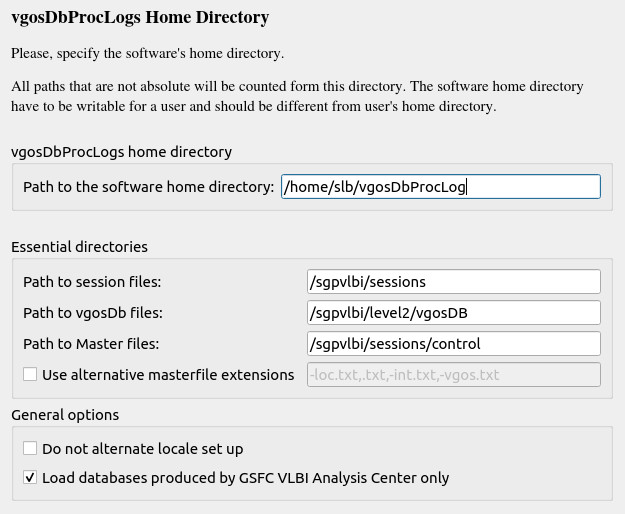
\includegraphics[width=0.6\textwidth]{wz-1-pl.jpg}
  \end{center}
  \caption{Setting up paths.}
  \label{fig-wizzard-1}
\end{figure}

The path to input default locations of station log files is in {\sl Path
to session files} filed. The data structure of the session files reflects
the data structure of the auxiliary files of the IVS web site
\begin{verbatim}
    https://cddis.nasa.gov/archive/vlbi/ivsdata/aux/
\end{verbatim}
The software expects in {\sl session} directory sub directories of the format
\begin{verbatim}
   <YYYY>/<SessionCode>/
\end{verbatim}
Where {\sl <YYYY>} is a four-digit year of observations and
{\sl <SessionCode>} is a code of a VLBI session as it appears in
corresponding master file.

The path to output directory is specified by the field {\sl Path to VgosDb files}.
The data structure of vgosDb files would looks like
\begin{verbatim}
   <VGOSDB_ROOT>/YYYY/YYMMMDDBL/<data files>
\end{verbatim}
Where {\sl VGOSDB\_ROOT} is a directory specified in the wizard and 
{\sl YYMMMDDBL} is a database name.

The software uses master files to figure out proper database name. Also,
the file {\sl ns-codes.txt} contains information on stations participated
in the observations. The path to master files is a place where these files
suppose to be. You can obtain the fresh copies of master files and
{\sl ns-codes.txt} file from
\begin{center}
{\tt
https://cddis.nasa.gov/archive/vlbi/ivscontrol/
}
\end{center}
\noindent
Time from time the files need to be updated. In addition to the standard master
files, a user can use its own "local" master file. The format of the local master
file should be the same as the standard one, its name have to be in the form
"masterYY-loc.txt", where "YY" -- two digits of the year. This feature is designed
for testing purposes or processing non-standard VLBI sessions. The software first
checks for the local master files, if it found a record there it stops the search,
so records in the canonical master files can be overwritten using the local
master file.

Starting with version 0.8.2 of the distribution, an option to expilictly set names
for master files is added. If a user sets the check box {\sl Use alternative
masterfile extensions} to <<on>>, then vgosDbProcLogs will compose the masterfile names
using a provided list of extensions. The list is a set of strings separated by
comma (","), colon (":") or semicolon (";") char. The software adds the extension
from the list to the basic name, "masterYY" or "masterYYYY", and reads such a file.
The order of files lookup is corresponding to the order of masterfile
extensions in the list. The default list of masterfile extensions is
"-loc.txt,.txt,-int.txt,-vgos.txt".

The check box {\tt Do not alternate locale set up} controls how the utility
deals with locale set up. By default it is <<off>>.

When a user loads a vgosDb database providing a session name, vgsDbCalc
usually reads the lates version of a wrapper file of the database.
However, sometimes it is preferrable to load the latest version produced
by your analysis center even if a higher version created by another
institution already exists. In this case turn on the checkbox
{\sl Load databases produced by [local] VLBI Analysis Center only}, where
[local] is an abbreviated acronym of your analysis center (see the next
subsection).


\section{Setting default cable calibration signs}
\label{config_cablecal_signs}
On the second page of the wizard a user can set up default cable calibration
sign for a station.

To determine a sign of obtained cable calibration measurements personnel
of a station performs the following operation: first, a cable calibration
measurement is performed. Then, an additional cable is inserted into cable
system of the antenna and the measurement is made again. Increase in cable
calibration reading with added piece of cable means that the sign of
the measurements is positive, otherwise it is negative. Such operation
usually is performed before begin and after end of a VLBI session and is
recorded into field system log of a station as \emph{cablelong} measurement.

Sometimes, for different reasons, such measurements are not conducted. In this
case vgosDbProcLogs use default cable calibration signs. A user can set up the
default sign for each station, see Fig.~\ref{fig-wizzard-5}. If a station is
not configured, a positive sign will be used.


\begin{figure}[htb!]
  \begin{center}
    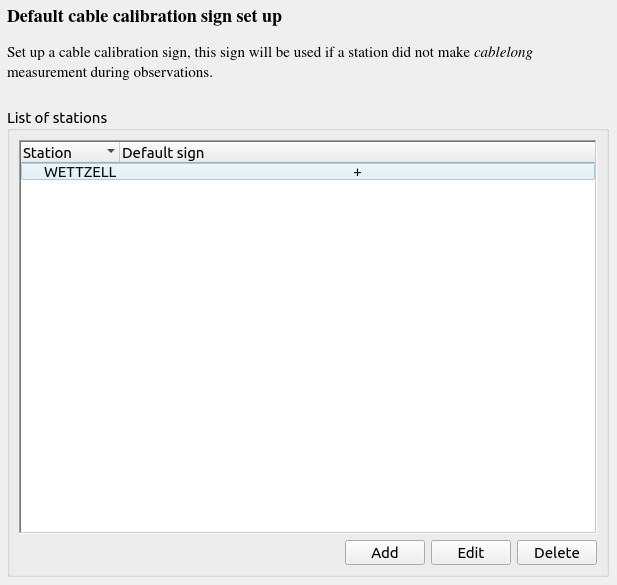
\includegraphics[width=0.6\textwidth]{wz-5-pl.jpg}
  \end{center}
  \caption{Setting up default cable calibration sign.}
  \label{fig-wizzard-5}
\end{figure}

By default, the station WETTZELL with the positive value for the cable calibration
sign is predefined.

\begin{figure}[htb!]
  \begin{center}
    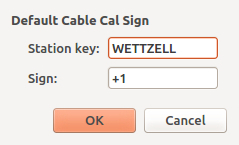
\includegraphics[width=0.3\textwidth]{wz-5-1-pl.jpg}
  \end{center}
  \caption{Editor of the default cable calibration sign.}
  \label{fig-wizzard-5-1}
\end{figure}

A user can edit existing station by clicking on the button <<Edit>>,
see Fig.~\ref{fig-wizzard-5-1}, add more stations (the button <<Add>>)
or remove existing stations from the configuration with the button <<Delete>>.




\section{Setting RINEX files}
\label{config_rinex}
The third page of the wizard allows a user to configure reading of RINEX files with
meteorological data.

The use of RINEX files as a source of meteorological data are described in
the Section~\emph{\ref{sect_using_rinex_files} Using RINEX files}. A user can
set up for each VLBI station its GPS counterpart and, if necessary, pressure
offset. The pressure offset could be necessary if meteo station and VLBI
antenna have difference in height and this difference is significant. Units for
the pressure offset are \emph{mbar}, the value will be added to the atmospheric
pressure extracted from RINEX files.

\begin{figure}[htb!]
  \begin{center}
    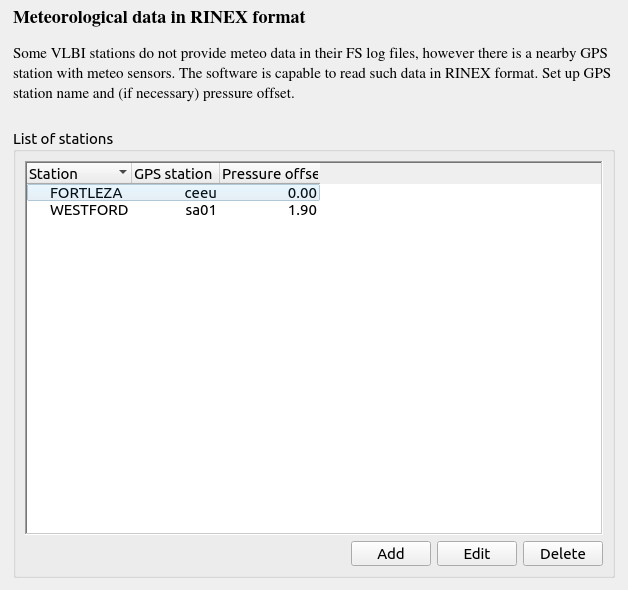
\includegraphics[width=0.6\textwidth]{wz-6-pl.jpg}
  \end{center}
  \caption{Setting up reading RINEX files.}
  \label{fig-wizzard-6}
\end{figure}

By default two stations are predefined: FORTLEZA with its nearby GPS station
<<ceeu>> and WESTFORD with the GPS station <<sa01>> and 1.90 mbar pressure offset.

\begin{figure}[htb!]
  \begin{center}
    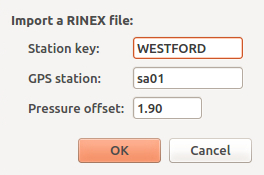
\includegraphics[width=0.3\textwidth]{wz-6-1-pl.jpg}
  \end{center}
  \caption{Editor of the using meteo data from RINEX files.}
  \label{fig-wizzard-6-1}
\end{figure}

A user can edit existing station by clicking on the button <<Edit>>,
see Fig.~\ref{fig-wizzard-6-1}, add more stations (the button <<Add>>)
or remove existing stations from the configuration with the button <<Delete>>.







\section{Setting user identities}
The fourth and fifth pages of the wizard, Fig.~\ref{fig-wizzard-2}-\ref{fig-wizzard-3},
set up user identities.

\begin{figure}[htb!]
  \begin{center}
    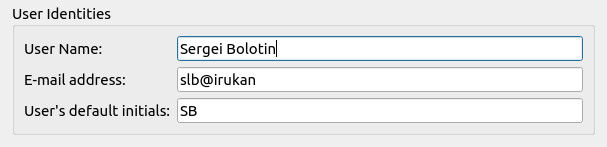
\includegraphics[width=0.6\textwidth]{wz-2.jpg}
  \end{center}
  \caption{Setting up user ID.}
  \label{fig-wizzard-2}
\end{figure}

%\section{Setting affiliation}

\begin{figure}[htb!]
  \begin{center}
    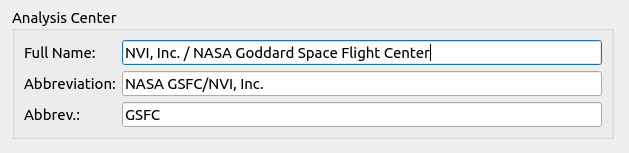
\includegraphics[width=0.6\textwidth]{wz-3.jpg}
  \end{center}
  \caption{Setting up affiliation.}
  \label{fig-wizzard-3}
\end{figure}

We strongly encourage users to provide, at least, a working e-mail
address.

Information collected by these two pages are used only for composing the
history part of vgosDb files and in vgosDbProcLogs log file.

The short form of the abbreviated affiliation (<<Abbrev.>> on the
Fig.~\ref{fig-wizzard-3}) is used in wrapper file names as an attribute
{\sl \_i<Institution>}. If the field is empty, the attribute will not be
added to a name of a wrapper file.



\section{Setting options of the logger}
\label{config_logger}
The last page of the start up wizard, Fig.~\ref{fig-wizzard-4}, sets up
properties of the logging subsystem. The field {\sl Log file name} is
a name of a file where the log messages will be saved if the checkbox
{\sl Save log to the file} is checked <<on>>. The file will appear in
vgosDbProcLogs home directory, Fig.~\ref{fig-wizzard-1}. The {\sl Log capacity}
is an amount of log records that are kept in internal structure before
send them to a file. The checkbox {\sl Put time stamps} turns on
adding time tags to the log messages.

\begin{figure}[htb!]
  \begin{center}
    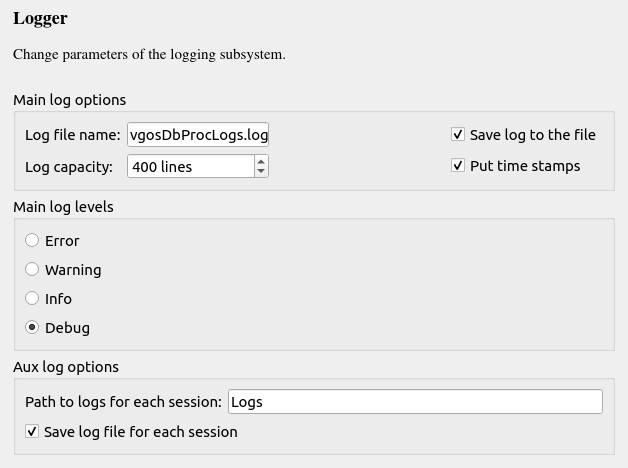
\includegraphics[width=0.6\textwidth]{wz-4-pl.jpg}
  \end{center}
  \caption{Setting up logger.}
  \label{fig-wizzard-4}
\end{figure}

The {\sl Log level} determines how verbose the log output will be. The {\sl Debug}
level, as shown on the figure, could be useful for debugging purposes. For
routine operations the {\sl Info} level will be preferred.

%The software does not control the size of the main log file, it will grow up
%with each invocation of the utility. A user should control the size of the log
%file and remove or back it up, what is necessary.

Another log file will be created on a per session basis if the checkbox
{\sl Save log file for each session} is turned <<on>>. The aux log file
will be saved in {\sl Path to logs for each session} directory and its
name will be the same as the database name plus ".log" extension.

{\bf \color{red}WARNING}: If the logger is instructed to save data in
the log file, the size of the file will grow up. The software does not
check the size of the file (it does not know about your intentions), and
eventually the file could take all free space on your computer! If you
do not need the log output from previous runs, please, remove the file on
a regular basis.




%%%%%%%%%%%%%%%%%%%%%%%%%%%%%%%%%%%%%%%%%%%%%%%%%%%%%%%%%%%%%%%%%%%%%%%%%%%%%%
%
%
\chapter{Concluding remark}
\label{chapt_concluding_remark}
Currently, this document is in the developmental stage, its content could change
time from time. Check for new versions at the site:

\begin{verbatim}
      https://sourceforge.net/projects/nusolve
\end{verbatim}

\noindent
If you have questions or suggestions that will improve the software or
the User Guide, please e-mail us at:

\begin{verbatim}
      <mailto:sergei.bolotin@nasa.gov>
\end{verbatim}

%\noindent
%Happy !


%%%%%%%%%%%%%%%%%%%%%%%%%%%%%%%%%%%%%%%%%%%%%%%%%%%%%%%%%%%%%%%%%%%%%%%%%%%%%%
%
%
\begin{thebibliography}{99}

\bibitem{Bolotin2010}
S. Bolotin, J. Gipson, D. MacMillan: ``Development of a New VLBI Data
Analysis Software". In: International VLBI Service for Geodesy and
Astrometry 2010 General Meeting Proceedings, edited by D. Behrend and K.
Baver, NASA/CP-2010-215864, 197-201, 2010.


\bibitem{Bolotin2011}
S. Bolotin, J. Gipson, D. Gordon, D. MacMillan: ``Current Status of
Development of New VLBI Data Analysis Software". In: Proceedings of the
20th Meeting of the European VLBI Group for Geodesy and Astrometry,
edited by W. Alef, S. Bernhart, A. Nothnagel, Schriftenreihe des
Instituts f\"ur Geod\"asie und Geoinformation der Universit\"at Bonn,
Nr. 22, ISSN 1864-1113, 86-88, 2011.


\bibitem{Bolotin2012}
S. Bolotin, K. Baver, J. Gipson, D. Gordon, D. MacMillan: ``The First
Release of $\nu$Solve". In: International VLBI Service for Geodesy and
Astrometry 2012 General Meeting Proceedings `Launching the
Next-Generation IVS Network', edited by D. Behrend and K. Baver,
NASA/CP-2012-217504, 222-226, 2012.


\end{thebibliography}


\end{document}


